\documentclass[t,aspectratio=169]{beamer}
\usepackage{modernbeamer}
\usepackage{tabularx}
\usepackage{booktabs}
\renewcommand{\tabularxcolumn}[1]{p{#1}}
\newcolumntype{Y}{>{\raggedright\arraybackslash\leavevmode}X}
\newcolumntype{H}{>{\raggedright\arraybackslash\leavevmode\bfseries\color{nlNavy}}p{3.5cm}}
\setlength{\aboverulesep}{0.7ex}
\setlength{\belowrulesep}{0.85ex}
\hyphenation{Hyderabad Bengaluru}
\usetikzlibrary{positioning}

\newtcolorbox{eqcard}[2][]{enhanced, colback=nlSurfaceWarm, colframe=nlBorder, boxrule=0.6pt,
  arc=3pt, boxsep=0pt, left=7pt, right=7pt, top=11pt, bottom=5pt, height=#2,
  fontupper=\footnotesize, fonttitle=\bfseries\footnotesize, coltitle=nlNavy, title={#1},
  attach boxed title to top left={yshift=-2mm, xshift=3mm},
  boxed title style={colback=nlBg, colframe=nlBorder, boxrule=0.5pt, arc=2pt,
    left=4pt, right=4pt, top=1.5pt, bottom=1.5pt}}

\newcommand{\person}[2]{%
  \node[draw=nlBorder, fill=nlSurfaceWarm, rounded corners=3pt, inner xsep=6pt, inner ysep=4pt,
        text width=2.55cm, align=left, font=\scriptsize] {\textbf{\color{nlNavy}#1}\\[-0.05em]{\tiny\color{nlMuted}#2}};}

\logo{
\includegraphics[height=0.90cm,keepaspectratio]{images/clglogo-cropped.png}}

\begin{document}

% 1 -------------------------------------------------------------------
\begin{frame}[c]
  \begin{center}
    {\scriptsize\bfseries\color{nlPrimary}CLOUD COMPUTING}\\[0.55em]
    {\fontsize{30}{34}\selectfont\jpmctitlefont\color{nlNavy}Zephyr}\\[0.15em]
    {\color{nlPrimary}\rule{2.6cm}{1.2pt}}\\[0.45em]
    {\footnotesize\color{nlText}Community Air Quality \& Environmental Health Dashboard}\\[0.7em]
    \begin{tikzpicture}
      \matrix[column sep=0.18cm, row sep=0.16cm, ampersand replacement=\&] {
        \person{Dhrushit Jain}{2023BCS-019} \&
        \person{Akshita Sure}{2023BCS-065} \&
        \person{Advay Bhagwat}{2023BCS-074} \\
      };
    \end{tikzpicture}\\[0.16em]
    \begin{tikzpicture}
      \matrix[column sep=0.18cm, ampersand replacement=\&] {
        \person{Apoorva Yadav}{2023BCS-076} \&
        \person{Nilanjan Mitra}{2023BCS-501} \\
      };
    \end{tikzpicture}\\[0.55em]
    
\includegraphics[height=1.15cm,keepaspectratio]{images/clglogo-cropped.png}
  \end{center}
\end{frame}

% 2 -------------------------------------------------------------------
\begin{frame}[c]{Why this exists}
  \begin{nlhighlight}[The gap]
    A station feed, a weather model, and a neighbour's complaint usually sit in three different products. A page that shows only the official monitor misses the plume the model sees, and the street someone just photographed.\\[0.3em]
    Zephyr is one site for all three. It follows twelve cities, draws the stations and the model on the same globe, and keeps a queue for the people who have to act on a report.
  \end{nlhighlight}
  \vspace{0.18cm}
  \begin{columns}[T,totalwidth=\textwidth]
    \begin{column}{0.48\textwidth}
      \begin{eqcard}[Show the air]{2.15cm}
        Delhi, Mumbai, Kolkata, Chennai, Bengaluru, Hyderabad, and six cities outside India. Each one has live stations, a wind field, and a CAMS heat layer on one map.
      \end{eqcard}
    \end{column}
    \hfill
    \begin{column}{0.48\textwidth}
      \begin{eqcard}[Crowdsource incident reports]{2.15cm}
        Residents file a photo and a hazard from where they stand. The worker reads the photo. Three reports that agree, or a sensor past its limit, open an incident for an operator.
      \end{eqcard}
    \end{column}
  \end{columns}
\end{frame}

% 3 -------------------------------------------------------------------
\begin{frame}[c]{What a user sees}
  \footnotesize
  \renewcommand{\arraystretch}{1.18}
  \begin{tabularx}{\textwidth}{@{}H Y@{}}
    \toprule
    \textcolor{nlNavy}{\textbf{Surface}} & \textbf{What it is for} \\
    \midrule
    Home & The city at a glance: the median, the band, how many stations are live, and which wards are being watched. \\
    Map & A globe. Pins for every city, a wind field, and a colour layer that can show US AQI or PM2.5. The overlay pauses while the map is moving. \\
    Zone & One station up close: the published index, the nearest monitor, the CAMS model, what is upwind, and a short advisory. \\
    Report & A photo and a hazard type, from a signed-in resident. The photo goes to Cloud Storage and the row waits for the worker. \\
    Operator & The incident queue. It opens only for an account whose \texttt{users.role} in Postgres is operator. \\
    \bottomrule
  \end{tabularx}
\end{frame}

% 4 -------------------------------------------------------------------
\begin{frame}[c]{Where the numbers come from}
  \begin{minipage}{\textwidth}
    \footnotesize The home page is not one sensor. Each city is a median of the stations that reported recently, and the map layers are separate feeds drawn on top of each other.
  \end{minipage}\par\vspace{0.3cm}
  \footnotesize
  \renewcommand{\arraystretch}{1.16}
  \begin{tabularx}{\textwidth}{@{}H Y@{}}
    \toprule
    \textcolor{nlNavy}{\textbf{Feed}} & \textbf{What we use it for} \\
    \midrule
    OpenAQ and WAQI & Station pollutants. The worker pulls them on a schedule and writes the rows the API serves. \\
    India AQI, US AQI & The city number, and the colour of the map. PM2.5 can be shown as a concentration instead of an index. \\
    Open-Meteo & Wind speed and direction, drawn as a field on the globe. \\
    CAMS & The model value on a zone page, and the heat layer behind the pins. \\
    Gemini & A reading of the resident's photo, so a report can be classified before it becomes an incident. \\
    \bottomrule
  \end{tabularx}
\end{frame}

% 5 -------------------------------------------------------------------
\begin{frame}[c]{From a photo to an incident}
  \begin{columns}[T,totalwidth=\textwidth]
    \begin{column}{0.48\textwidth}
      \begin{eqcard}[What the resident does]{4.7cm}
        They sign in, pick a hazard, and attach a photo. The report is tied to that account, not to a shared inbox.\\[0.45em]
        Nothing is published to the operator queue at this moment. The photo and the row are stored, and the API hands the job to the worker.
      \end{eqcard}
    \end{column}
    \hfill
    \begin{column}{0.48\textwidth}
      \begin{eqcard}[What the worker decides]{4.7cm}
        Gemini classifies the photo. The worker then looks for corroboration: three reports that agree, or a nearby sensor over its limit.\\[0.45em]
        Either of those can open an incident. An operator, flagged in the database rather than in an allowlist, works the queue.
      \end{eqcard}
    \end{column}
  \end{columns}
\end{frame}

% 6 -------------------------------------------------------------------
\begin{frame}[c]{What it is built with}
  \footnotesize
  \renewcommand{\arraystretch}{1.12}
  \begin{tabularx}{\textwidth}{@{}H Y@{}}
    \toprule
    \textcolor{nlNavy}{\textbf{Layer}} & \textbf{Choice} \\
    \midrule
    Language & TypeScript. A Bun 1.4 workspace: \texttt{apps/web}, \texttt{apps/api}, \texttt{apps/worker}, plus \texttt{@zephyr/domain} and \texttt{@zephyr/server}. \\
    Web & React 19, Vite, MapLibre, React Router, and the Firebase client. The production build is hosted on Vercel. \\
    API & Express on Bun. In production it is the Cloud Run service \texttt{zephyr-api}, and Vercel rewrites \texttt{/api} to it. \\
    Worker & A second Bun service, \texttt{zephyr-worker}. It ingests, classifies, and writes. It is not publicly invokable. \\
    Data & PostgreSQL 16. Cloud SQL in production, Postgres in Docker for local work. Objects go to Cloud Storage, or to MinIO locally. \\
    Auth & Google Identity Platform. The web uses the Firebase client. The API checks the ID token. \\
    \bottomrule
  \end{tabularx}
\end{frame}

% 7 -------------------------------------------------------------------
\begin{frame}[c]{Terraform is the project}
  \begin{minipage}{\textwidth}
    \footnotesize The GCP project is not assembled in the console. \texttt{infra/terraform} is the source, with the Google provider 6.x, project \texttt{zephyr-512319}, region \texttt{asia-south1}.
  \end{minipage}\par\vspace{0.3cm}
  \footnotesize
  \renewcommand{\arraystretch}{1.14}
  \begin{tabularx}{\textwidth}{@{}H Y@{}}
    \toprule
    \textcolor{nlNavy}{\textbf{What apply creates}} & \textbf{Why it is there} \\
    \midrule
    Cloud Run & The API and the worker, plus Artifact Registry for the images they run. \\
    SQL and storage & Cloud SQL for the database. Cloud Storage for photos, the wind grid, and the model image. \\
    Secrets and login & Secret Manager for keys and the database URL. Identity Platform for email and password on this project. \\
    Jobs and queues & Pub/Sub for \texttt{report.submitted}, Cloud Scheduler for the four timed jobs, Cloud Tasks for alerts. \\
    IAM and history & One service account each for the API, the worker, the scheduler, and Pub/Sub push. BigQuery for station history. \\
    \bottomrule
  \end{tabularx}
\end{frame}

% 8 -------------------------------------------------------------------
\begin{frame}{How the deployment is wired}
  \vspace{-0.45cm}
  \begin{center}
    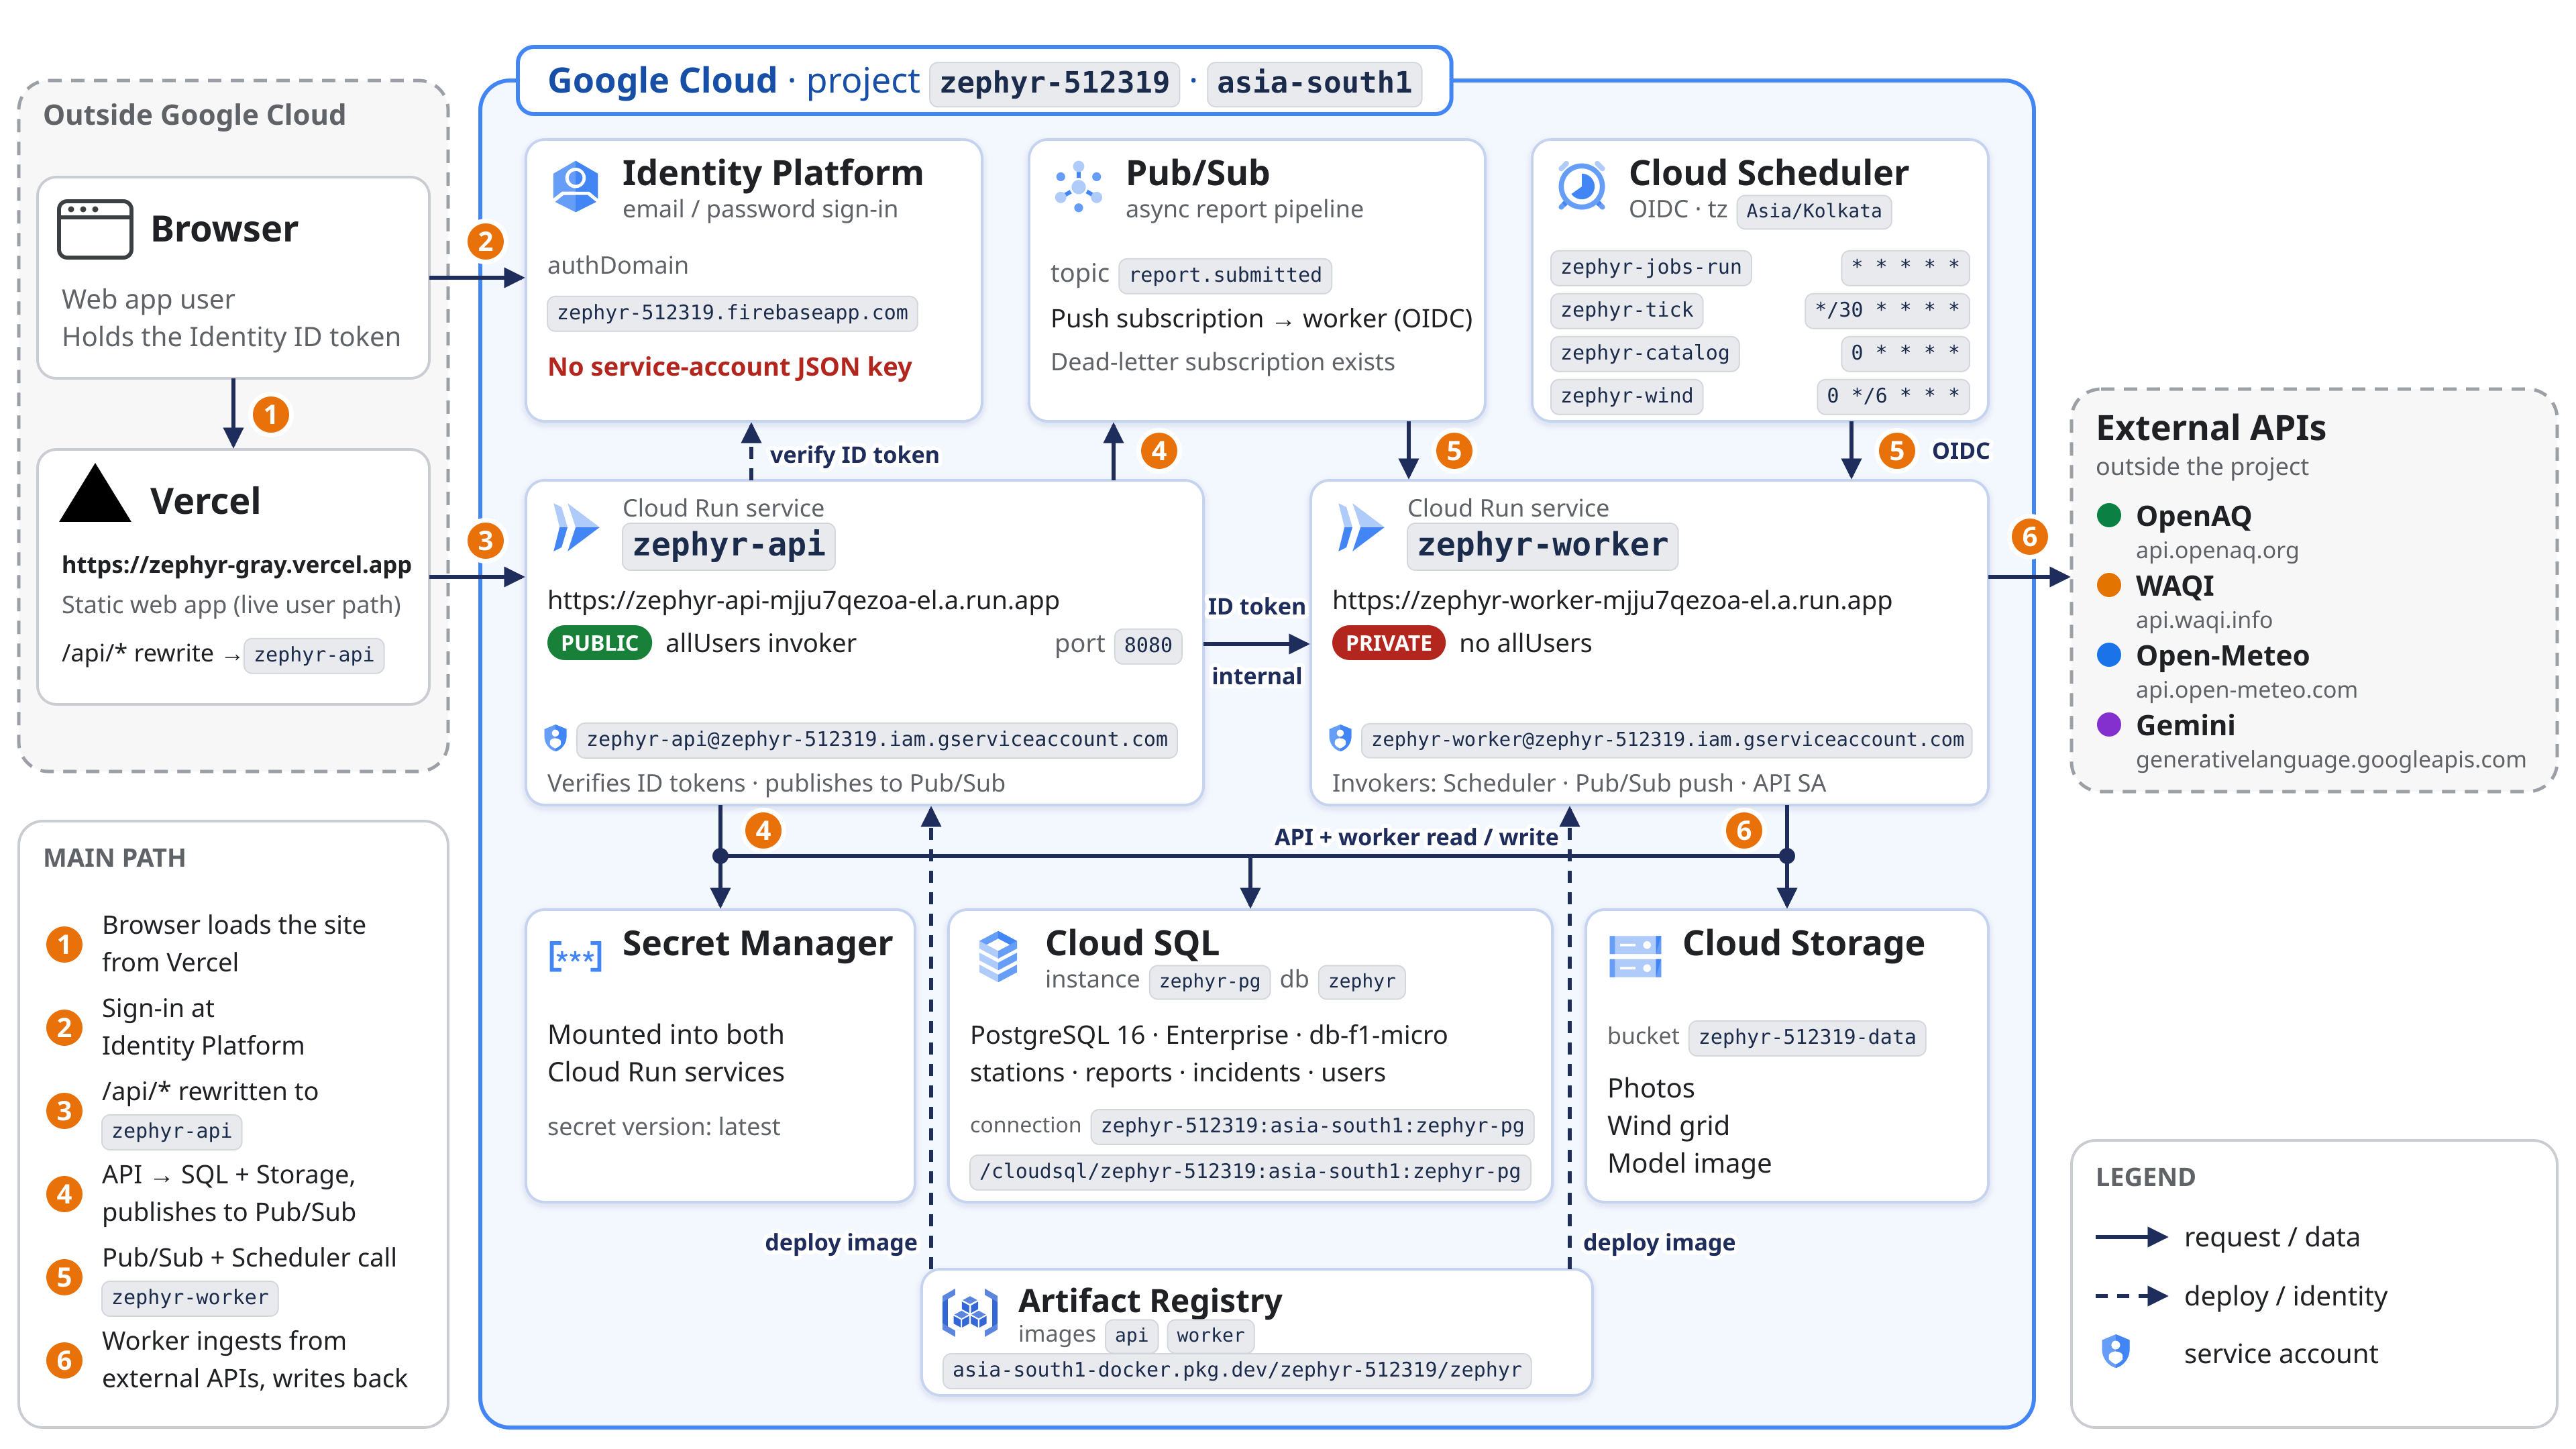
\includegraphics[width=\textwidth,height=0.84\textheight,keepaspectratio]{images/gcp-deploy.png}
  \end{center}
\end{frame}

% 9 -------------------------------------------------------------------
\begin{frame}[c]{One request, and one tick}
  \begin{columns}[T,totalwidth=\textwidth]
    \begin{column}{0.48\textwidth}
      \begin{eqcard}[A resident report]{4.85cm}
        \begin{enumerate}
          \item Identity Platform issues a token. The API checks it on every call.
          \item The client posts the report, then the photo, then commits.
          \item The photo lands in Cloud Storage. The row lands in Cloud SQL.
          \item The API publishes \texttt{report.submitted}.
          \item Pub/Sub pushes the worker, which classifies the photo and may open an incident.
        \end{enumerate}
      \end{eqcard}
    \end{column}
    \hfill
    \begin{column}{0.48\textwidth}
      \begin{eqcard}[Cloud Scheduler]{4.85cm}
        \begin{enumerate}
          \item Every minute, a job asks the worker to drain whatever is queued.
          \item Every 30 minutes, a tick enqueues the twelve cities.
          \item The station catalog runs hourly. The wind grid runs every six hours.
          \item The worker pulls OpenAQ and WAQI, writes SQL, and stores the wind grid and the model image in Cloud Storage.
        \end{enumerate}
      \end{eqcard}
    \end{column}
  \end{columns}
\end{frame}

% 10 ------------------------------------------------------------------
\begin{frame}[c]{Who can call what, and where state sits}
  \begin{columns}[T,totalwidth=\textwidth]
    \begin{column}{0.48\textwidth}
      \begin{eqcard}[Who may do what]{4.55cm}
        An operator is a row in Postgres, \texttt{users.role}, not a list of emails in the environment. Until that flag is set, the account is a resident.\\[0.4em]
        The worker accepts calls only from identities that hold \texttt{run.invoker}: Cloud Scheduler, the Pub/Sub push account, and the API. The API presents a Google identity token.
      \end{eqcard}
    \end{column}
    \hfill
    \begin{column}{0.48\textwidth}
      \begin{eqcard}[Where state lives]{4.55cm}
        Cloud SQL holds stations, reports, incidents, and users. Cloud Storage holds photos, the wind grid, and the model image.\\[0.4em]
        Secret Manager holds OpenAQ, WAQI, Gemini, and the database URL. Both Cloud Run services mount the latest version. No service-account JSON key is stored. The organisation blocks those keys.
      \end{eqcard}
    \end{column}
  \end{columns}
\end{frame}

% 11 ------------------------------------------------------------------
\begin{frame}[c]{What is live}
  \footnotesize
  \renewcommand{\arraystretch}{1.16}
  \begin{tabularx}{\textwidth}{@{}H Y@{}}
    \toprule
    \textcolor{nlNavy}{\textbf{Piece}} & \textbf{Where it runs} \\
    \midrule
    Web & \mbox{\texttt{zephyr-gray.vercel.app}}. \texttt{/api} is rewritten to Cloud Run. \\
    API & Cloud Run \texttt{zephyr-api}, public invoker, container port 8080. \\
    Worker & Cloud Run \texttt{zephyr-worker}. Scheduler, Pub/Sub, and the API are the only callers. \\
    Database & Cloud SQL Postgres 16, instance \texttt{zephyr-pg}, database \texttt{zephyr}. \\
    Objects & Bucket \mbox{\texttt{zephyr-512319-data}}. Images in Artifact Registry, region \mbox{\texttt{asia-south1}}. \\
    Login & Identity Platform on \texttt{zephyr-512319}. \\
    \bottomrule
  \end{tabularx}
  \vspace{0.28cm}
  {\footnotesize After the first tick, Delhi's median was 368, from 18 live stations. OpenAQ, WAQI, and Gemini are configured.}
\end{frame}

% 12 ------------------------------------------------------------------
\begin{frame}[c]
  \begin{center}
    {\fontsize{30}{34}\selectfont\jpmctitlefont\color{nlNavy}Thank you}\\[0.25em]
    {\color{nlPrimary}\rule{2.6cm}{1.2pt}}\\[0.85em]
    {\scriptsize\color{nlMuted}%
      Dhrushit Jain \quad Akshita Sure \quad Advay Bhagwat\\[0.28em]
      Apoorva Yadav \quad Nilanjan Mitra}\\[0.9em]
    
\includegraphics[height=1.15cm,keepaspectratio]{images/clglogo-cropped.png}
  \end{center}
\end{frame}

\end{document}
